\section{Objective}

The aim of this project is to develop an application which creates an undistorted image from a distorted image. This means that the distorted image with its non-straight edges should be transformed into an undistorted image, where the non-straight edges are straightened.\\ 

Distorted images are naturally generated by the camera because of its lens properties. It cannot be assumed that even cameras of the same model have the exact same lens properties. That's why it is important to calibrate every camera for its intrinsic matrix, which can be used to undistort the images. \cite{cv}\\

To achieve this goal in this project, recordings have been provided as a source which show an 8x8 chessboard. In these, the chessboard is placed by a person in different positions and at different angles to the camera. These frames in the recordings are the basis for the camera calibration.\\
\vspace{-2mm}
\begin{wrapfigure}{L}{0.57\textwidth}
    \centering
     \captionsetup{justification=centering}
     \vspace{-4mm}
     \begin{minipage}[b]{0.55\textwidth}
         \centering
         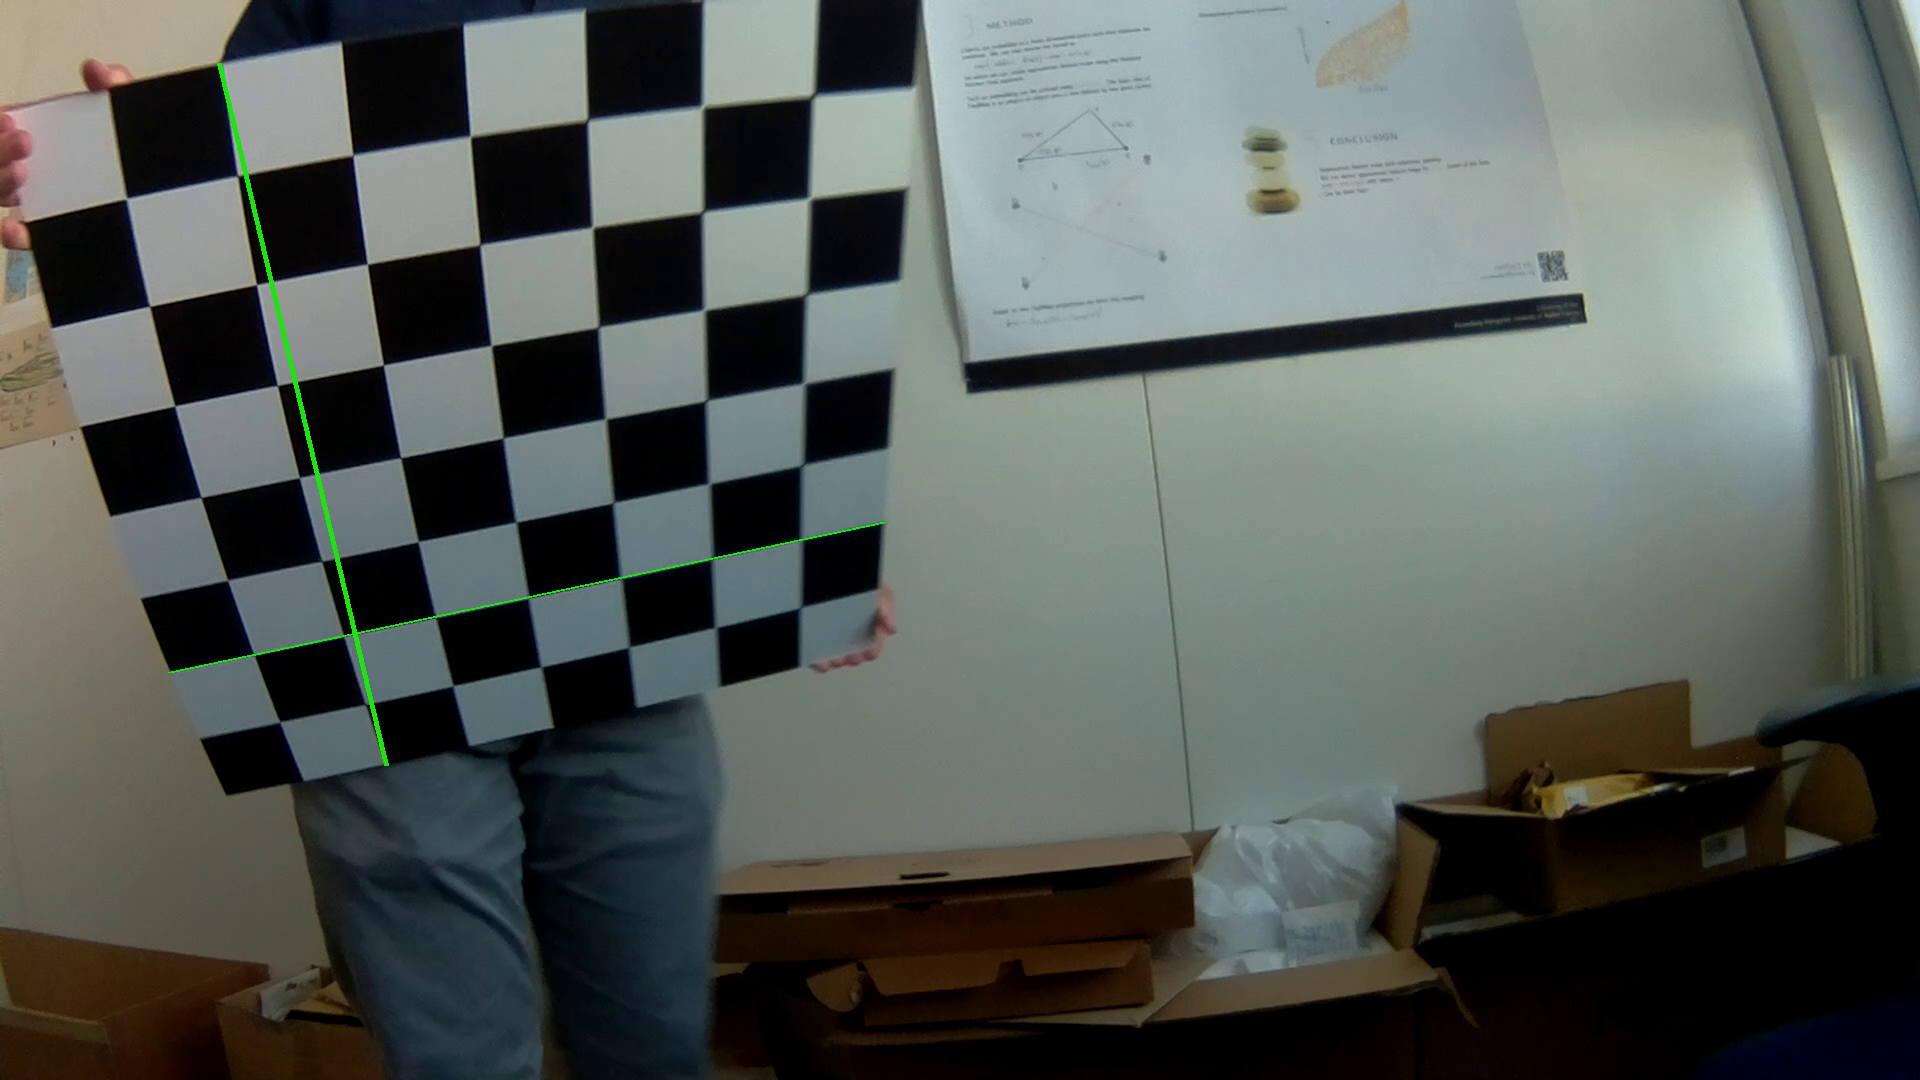
\includegraphics[width=\textwidth]{image/1/og.png}
         \caption{Distorted (original) frame from the source recording}
         \label{fig:og_frame}\par
         \vspace{6mm}
         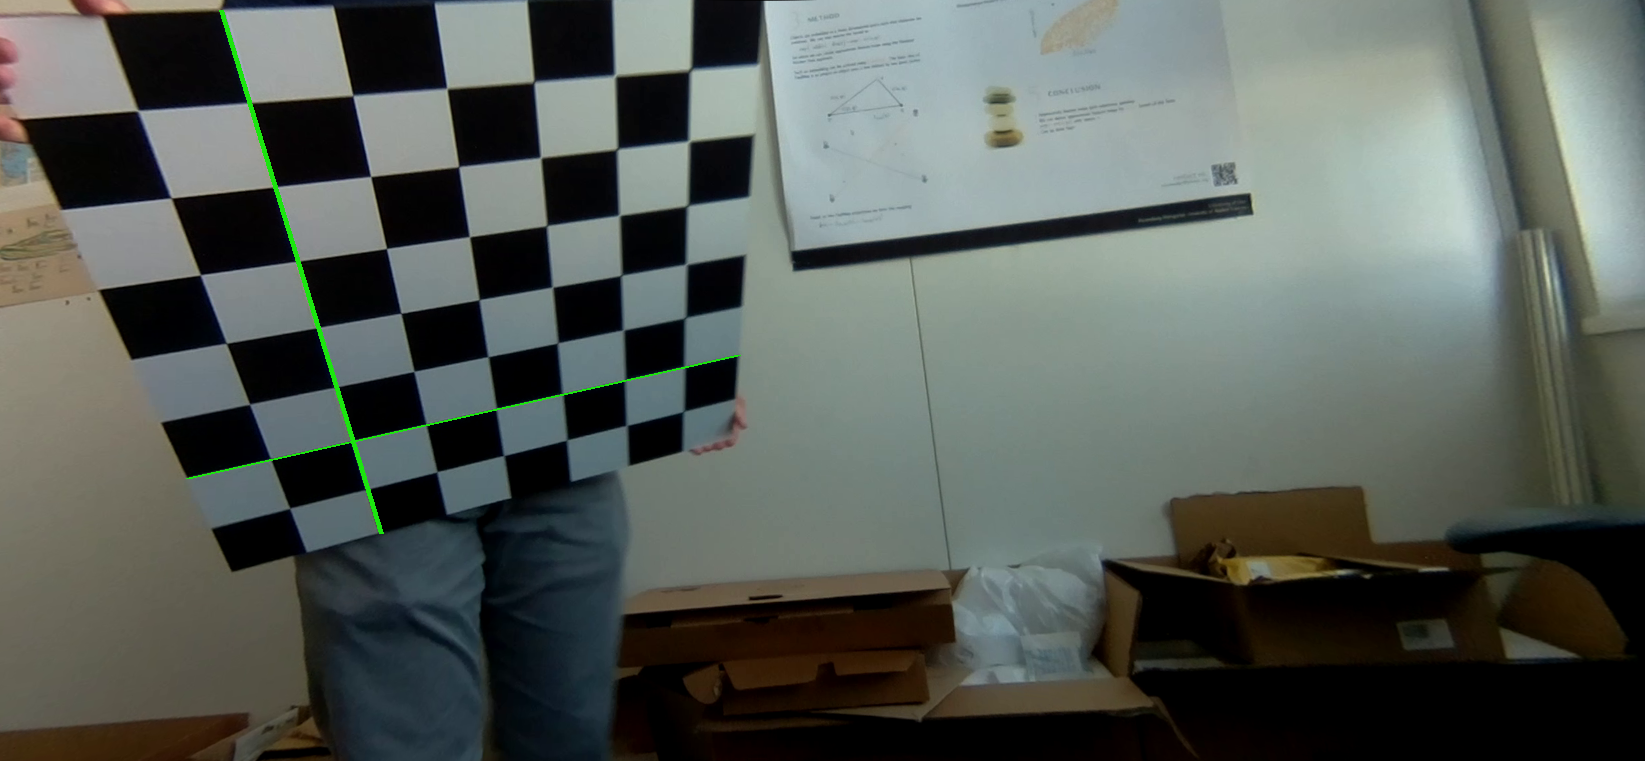
\includegraphics[width=\textwidth]{image/1/undist.png}
         \caption{Undistorted frame}
         \label{fig:dst_frame}
     \end{minipage}
     \hfill
     \vspace{-9mm}
\end{wrapfigure}

Figure \ref{fig:og_frame} shows an example frame of the recording and figure \ref{fig:dst_frame} the undistorted image of the distorted frame. The straight green line should serve as a reference to compare the non-straight edges to the straight edges of the checkerboard in the images.\\

The additional goals for this project are:
\begin{enumerate}[leftmargin=0.9cm]
    \item Provide all intrinsic camera parameters.
    \item Provide the distortion coefficients and generate the undistorted images for at least four different images from each video. Compare them to the original and distorted images.
\end{enumerate}

\newpage
